\chapter{Untersuchung von MorphNet}\label{sec:morphexperimente}
\color{blue1}

Die in Kapitel \ref{sec:morphnet} erläuterte Methode zum ``schnellen Ressourcen beschränkten Strukturlernen'' (MorphNet) wird in diesem Kapitel evaluiert. In Algorithmus \ref{alg:morphnet} wird das Vorgehen von MorphNet mittels Pseudocode dargestellt. Im ersten Schritt zur Evaluierung werden die einzelnen Schritte in diesem Algorithmus evaluiert. Im zweiten Schritt wird dann überprüft, wie gut der Algorithmus mit den in Kapitel \ref{sec:konzept} genannten Rahmenbedingungen abschneidet. Da für ide Untersuchung der einzelnen Schritte von MorphNet die Ausführungszeit unwichtig ist wird dieser Teil auf der Geforce GTX 1080 Ti ausgeführt.


\section{Evaluierung der einzelnen Schritte von MorphNet}
Im ersten Schritt von MorphNet wird das Netz trainiert um $\mathcal{W}^{\ast}=\underset{\mathcal{W}}{arg min}\; l(f(\mathbf{x_i}, \mathcal{W},y_i) + \lambda \mathcal{G}(\mathcal{W}))$. Der Regularisierer $\mathcal{G}$ ist in dieser Formel dafür zuständig, dass die gewählte Zielgröße minimiert wird. Die zwei möglichen Zielgrößen sind die Modellgröße und Anzahl an FLOPs. Für beide Zielgrößen gilt, dass die im Regularsierer verwendete Formel nur eine vereinfachte Form der Zielgrösse berechnet. In Abbildung \ref{abb:morphSize} ist in Blau abgebilder, wie sich der Wert des Regularisieres währendem Training verändert, Die grüne Kurve in Abbildung \ref{abb:morphSize} ist der tatsächliche Verlauf der Modellgröße über die Trainingszeit. Da beide Kurven einen ähnlichen Verlauf und eine ähnliche Krümmung zeigen berechnet $\mathcal{G}$ zwar eine vereinfachte Form der Zielgröße minimiert aber auch die Zielgröße. 
Für die Zielgröße FLOPs ist der Verlauf der beiden Kurven in Abbildung \ref{sec:morphFLOPs} abgebildet. Auch hier kann die gleiche Aussage wie zur Modelgröße getroffen werden.

\begin{figure}
     \centering
     \subfloat[][]{\missingfigure{Size}\label{abb:morphSize}}
     \hfill
     \subfloat[][]{
     \missingfigure{Size}\label{abb:morphFLOPs}
     %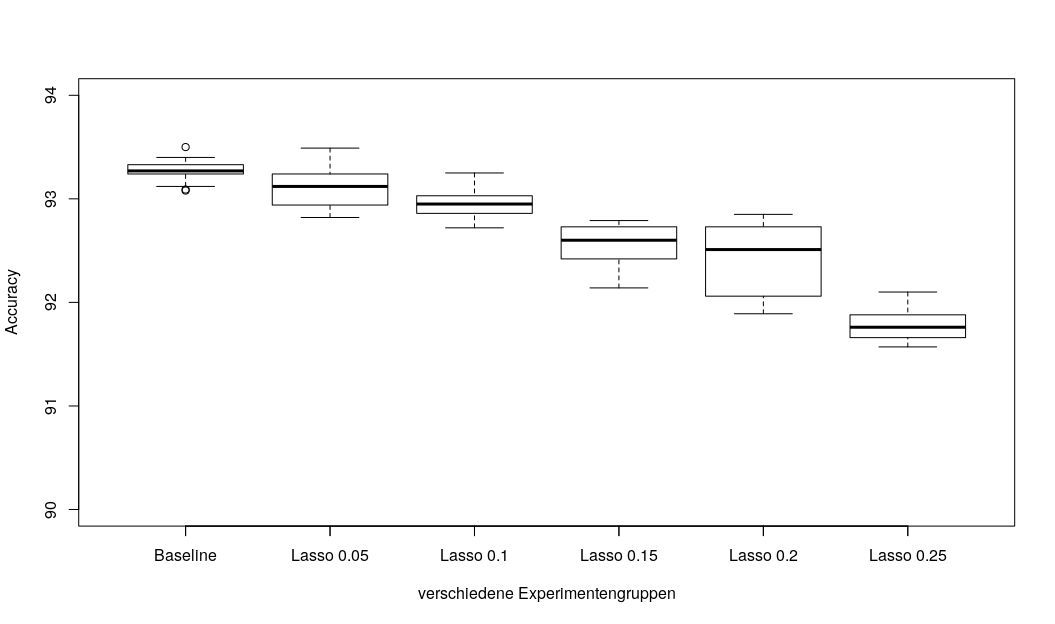
\includegraphics[width=.5\linewidth]{KapitelPartB/Images/lasso2.png}\label{abb:lasso2}
     }
     \caption{Vergleich Zielgröße mit Wert des Regularisierers für (a) Modellgröße (b) FLOPs}
     \label{abb:morph1}
\end{figure}



Als weiteren Schritt in der Evaluation des MorphNets wird der Effekt von unterschiedlichen Werten für $\lambda$ untersucht. Zu diesen Zweck wird ein Netzwerk mit verschiedenen Werten für $\lambda$ trainiert.   



\section{Evaluierung der Ergebnisse von MorphNet}


Danach wird evaluiert wie aus einem ResNet 32 mit Anfangsbreite ein grösseres Netz wird. Erlaubt sind maximal die Flops/bzw. Modelgrösse des 16 breiten Netzwerks






\color{black}





\chapter{Evaluation des Beschneidens des Netzes}\label{sec:ptexperimente}
\section{Evaluation bei gleichbleibender Batchgröße}
Die Untersuchung von PruneTrain basiert auf einer bereits vorgefertigten Implementierung \cite{ptImpl}. In dieser Implementierung ist alles bis auf die Anpassung der Batchgröße an das kleiner werdende Netz enthalten. Es wird das Ergebnis der Ausführung von PruneTrain auf der Hardware mit den Ergebnissen aus der Veröffentlichung verglichen \cite{prunetrain}. Ziel der Experimente ist es zu evaluieren, wie eine Änderung der verschiedenen Hyperparameter die Trainingszeit und die Accuracy beeinflusst. Im Gegensatz zur Veröffentlichung von PruneTrain wird hier statt auf mehreren GPUs nur auf einer GPU gerechnet. Bei der Evaluierung der Einflüsse werden die veränderbaren Hyperparameter von PruneTrain einzeln verändert, um den Einfluss der einzelnen Veränderungen zu untersuchen.  
Die veränderbaren Hyperparameter sind:
\begin{itemize}
 \item Lasso-Ratio $0,2$
 \item Rekonfigurationsinterval $5$
 \item Grenzwert $0,0001$
 \item Lernrate $0,1$
\end{itemize}
Hinter den veränderbaren Hyperparameter steht jeweils der Wert, den der Hyperparameter hat, wenn er im aktuellen Experiment nicht verändert wird, hat.
Betrachte eine feste Batchgröße von 256 über 180 Epochen und vergleiche diese mit dem Baseline-Netzes aus Kapitel \ref{sec:baseline}. 


\subsubsection{Einfluss von verschiedenen Lasso-Ratio Werten auf das Netz}
\color{vermi}
Die Lasso-Ratio gibt an, wie stark das Netz beschnitten werden soll. In diesen Experimenten wird die Lasso-Ratio von 0,05 bis 0,25 in 0,05er Schritten verändert. In Abbildung \ref{abb:lasso1} ist zusehen, dass mit steigender Lasso-Ratio durchschnittlich weniger Trainingszeit gebraucht wird. Für die durchschnittliche Trainingszeit einer Epoche wird das arithmetische Mittel über alle Epochen angewandt. Die Experimente werden dann nach ihrer Zugehörigkeit einsortiert und als Boxplot in Abbildung \ref{abb:lasso1} dargestellt. Trotz der nachlassenden Trainingszeit mit steigender Lasso-Ratio ist die Trainingszeit des Baseline-Netzes signifikant schneller. Dies ist durch den Overhead erklärbar, welcher durch das Beschneiden des Netzes entsteht.


In Abbildung \ref{abb:lasso2} ist die Accuracy der verschiedenen Experimente abgebildet. Es fällt auf, dass das Baseline-Netz im Mittel etwa schlechter ausfällt als die Experimente mit den Lasso-Ratio von 0,05 bis 0,15. Der Grund hierfür ist ein Overfitting. Das Overfitting wurde hier erkannt durch eine Trainingsaccuracy von 100,00 \% für mehrere Epochen ohne ein weiter steigende Validierungsaccuracy. 
\begin{figure}
     \centering
     \subfloat[][]{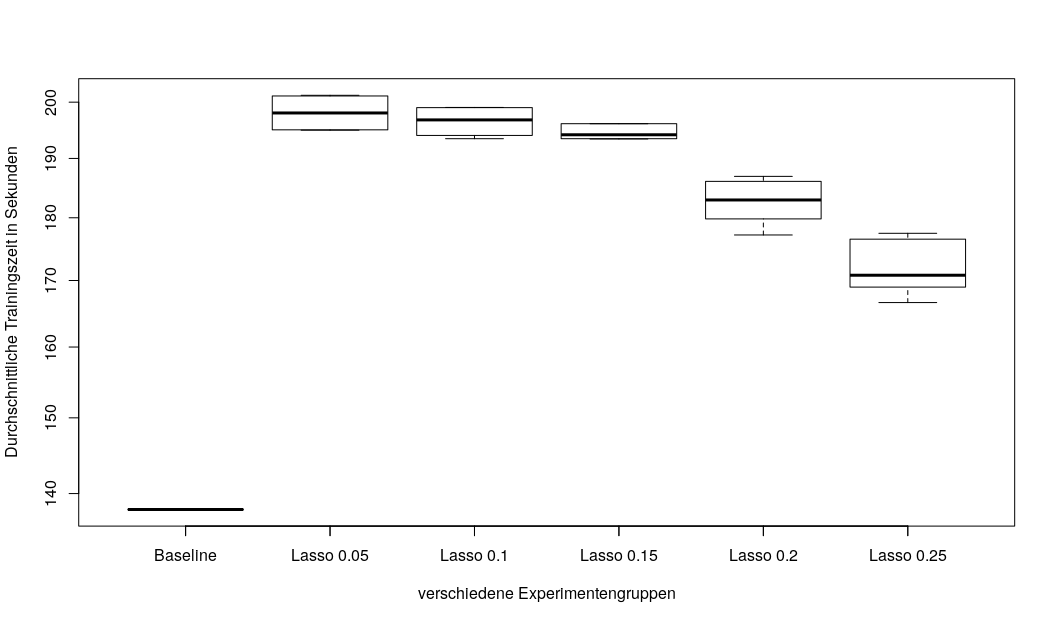
\includegraphics[width= .5\linewidth]{KapitelPartB/Images/lasso1.png}\label{abb:lasso1}}
     \hfill
     \subfloat[][]{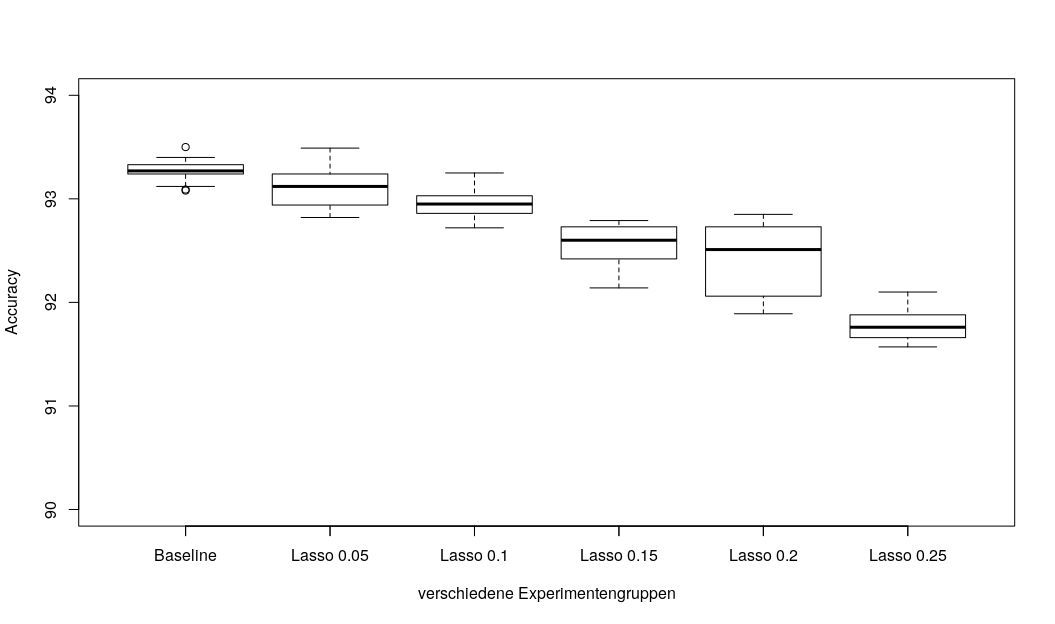
\includegraphics[width=.5\linewidth]{KapitelPartB/Images/lasso2.png}\label{abb:lasso2}}
     \caption{Lasso-Ratio Experiment: (a) Boxplot der durchschnittlichen Trainingszeit (b) Boxplot der Accuracys}
     \label{abb:lasso}
\end{figure}




\subsubsection{Experimente zum Rekonfigurationsintervall}
 Als nächste Größe wird der Einfluss des Rekonfigurationsintervalls überprüft. Die entsprechenden Grafiken sind in Abbildung \ref{abb:reconf} zu sehen. In Abbildung \ref{abb:reconf1} sind für die verschiedenen Experimente die Trainingszeiten pro Epoche zu sehen. Dabei werden drei verschiedene Rekonfigurationsintervalle (2,5 und 10) verglichen. In Abbildung \ref{abb:reconf1} lässt sich für die verschiedenen Trainingszeiten der Experimente zum Rekonfigurationsintervall kaum Unterschiede erkennen. Daher ist in Abbildung \ref{abb:reconf3} ein Boxplot ohne die Baseline Werte abgebildet. 
 
 
\begin{figure}
     \centering
     \subfloat[][]{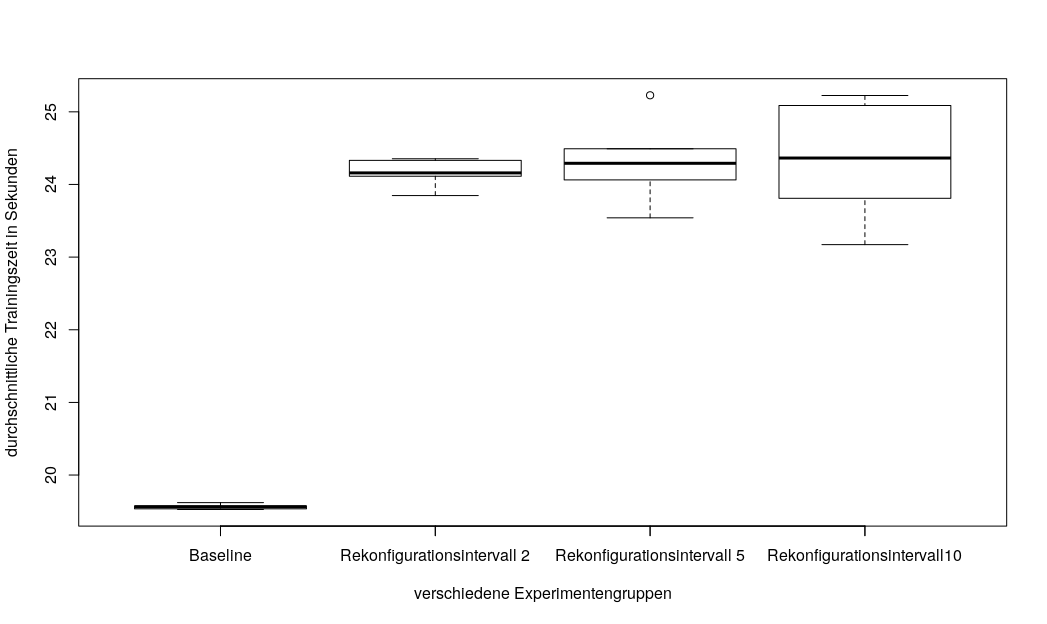
\includegraphics[width= .45\textwidth]{KapitelPartB/Images/reconf1.png}\label{abb:reconf1}}
     \hfill
     \subfloat[][]{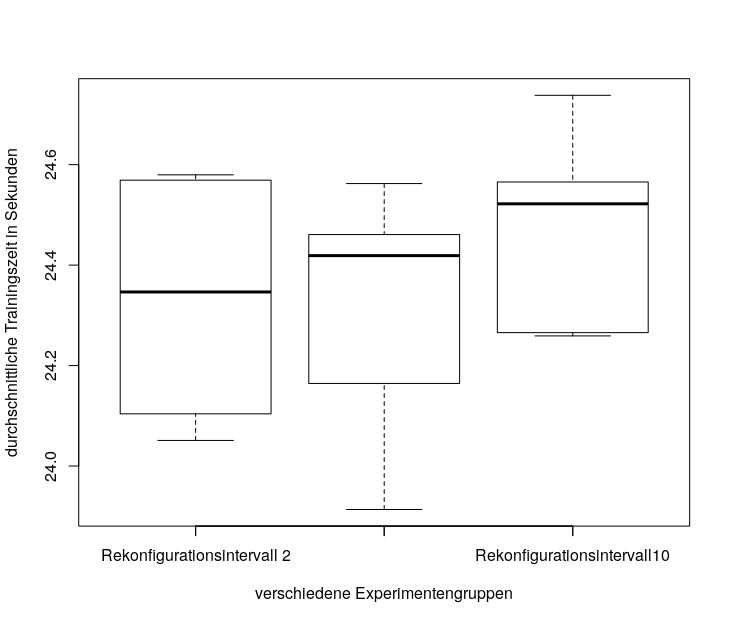
\includegraphics[width= .45\textwidth]{KapitelPartB/Images/reconf3.png}\label{abb:reconf3}}
     \\
     \subfloat[][]{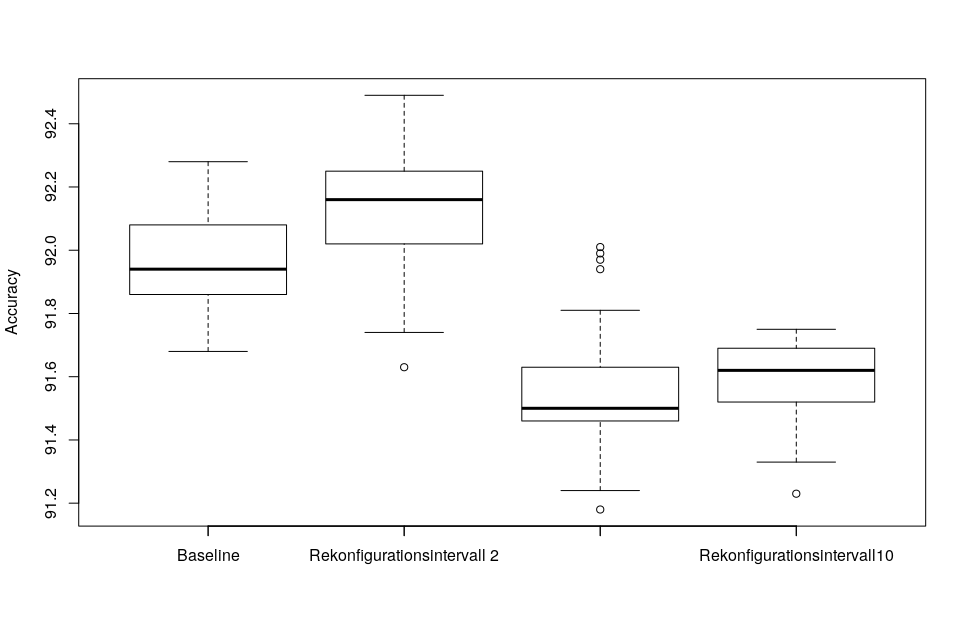
\includegraphics[width=.45\textwidth]{KapitelPartB/Images/reconf2.png}\label{abb:reconf2}}
     \caption{Experimente zum Rekonfigurationsintervall: (a) Boxplot der durchschnittlichen Trainingszeit (b) Boxplot der durchschnittlichen Trainingszeit ohne Baseline-Netz (c) Boxplot der Accuracys}
     \label{abb:reconf}
\end{figure}

 Mit Hilfe dieses Boxplots lässt sich erkennen, dass die durchschnittliche Trainingszeit aller Experimente mit dem Rekonfigurationsintervall steigt.
 
 In Abbildung \ref{abb:reconf2} ist zu sehen, wie sich die Accuracy bei diesen Experimenten verhält.
 \todo[inline]{Die Effekte in der Accuracy vom Baseline Netz zum Rekonfigurationsintervall sind wieder mit einem Overfitting zu erklären. Die Effekte vom Rekonfigurationsinterval 2 zu 5 und zu 10 sind auch mit Zunehmenden Overfitting je weniger geprunt wird zu erklären. Abhilfe mehr Experimente und zwar mit dem schmallen Baseline Netz}
 
\subsubsection{Experimente zur Lernrate}
Der Einfluss der Lernrate auf das Beschneiden des Netzes wird mit fünf verschiedenen Lernraten untersucht. Beginnend mit der Lernrate $0,2$ und für jede weitere der fünf Lernraten die Hälfte der vorherigen.
Die durchschnittliche Trainingszeit in Sekunden für verschiedene Lernrate ist in Abbildung \ref{abb:lr} zu sehen. Es ist deutlich zu sehen, dass mit sinkender Lernrate die Trainingszeit steigt. Das bedeutet, dass mit sinkender Lernrate weniger von Netz beschnitten wird.
 
 \begin{figure}
     \centering
     \subfloat[][]{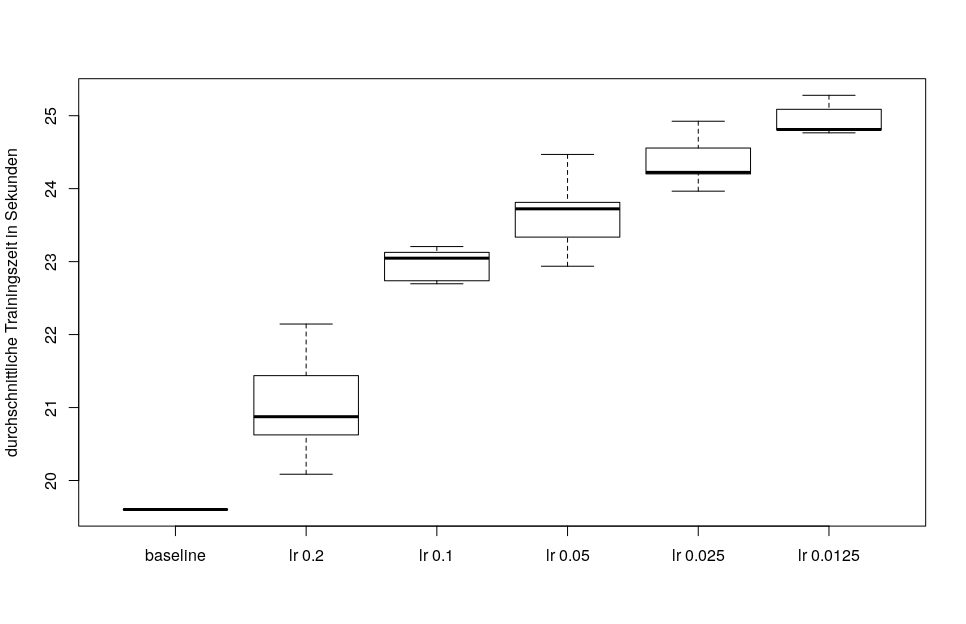
\includegraphics[width= .45\textwidth]{KapitelPartB/Images/lr1.png}\label{abb:lr1}}
     \hfill
     \subfloat[][]{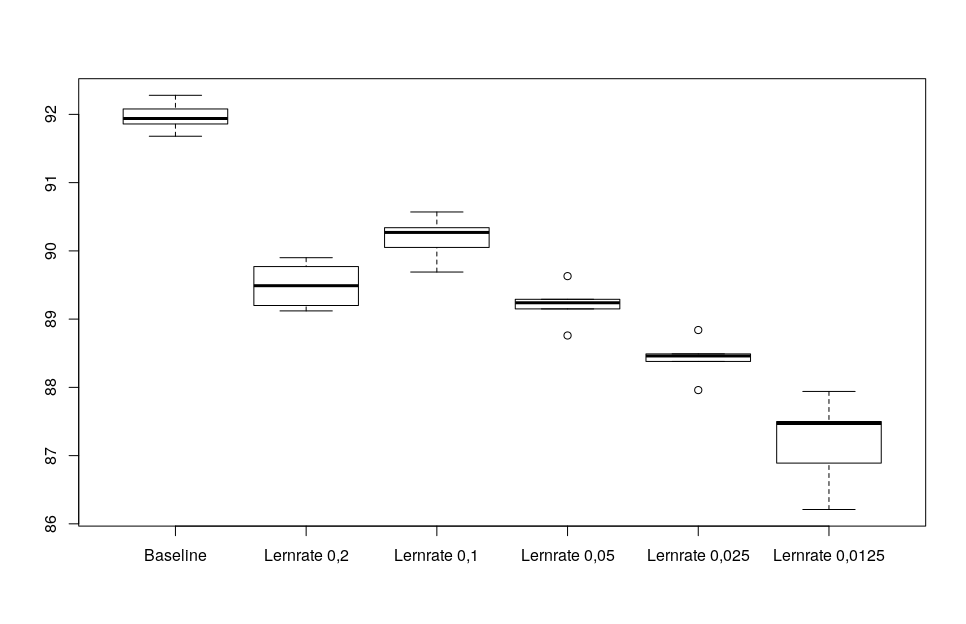
\includegraphics[width= .45\textwidth]{KapitelPartB/Images/lr2.png}\label{abb:lr2}}
     \caption{Experimente zuLernrate: (a) Boxplot der durchschnittlichen Trainingszeit (b) Boxplot der durchschnittlichen Trainingszeit ohne Baseline-Netz (c) Boxplot der Accuracys}
     \label{abb:lr}
\end{figure}

 In Abbildung \ref{abb:lr2} sind die Accuracy der verschiedenen Lernrate abgildet. Die Lernrate $0.1$ schneidet hier am Besten ab. Dies kann darauff zurück geführt werden, dass bei einer größeren Lernrate weniger Minima in der Verlustfunktion gefunden werden können. Der Effekt bei wesentlich kleineren Lernraten ist, dass der Trainingsprozess zwar mit jedem Schritt in die Richtung des Minimums geht, dabei aber durch die kleine Lernrate das tatsächliche Minimum innerhalb der 180 Epochen nicht erreicht.
 
 
 
 \subsubsection{Experimente zum Grenzwert}


\begin{figure}[h]
 \centering
 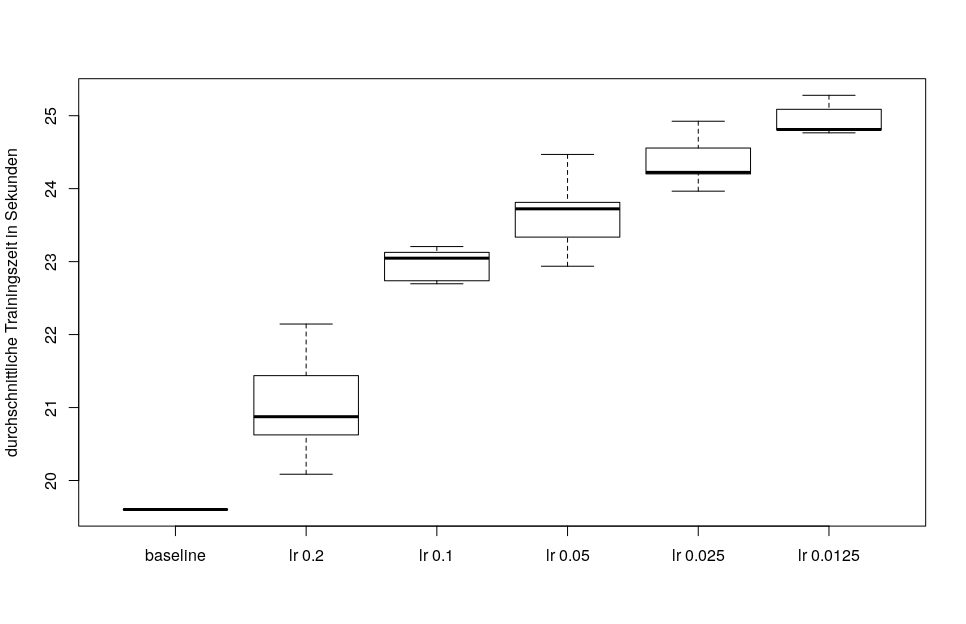
\includegraphics[width=0.8\textwidth]{KapitelPartB/Images/lr1.png}
 % lr1.png: 431x491 px, 96dpi, 11.41x12.99 cm, bb=0 0 323 368
 \label{ref:lra}
\end{figure}



 

\subsubsection{Diskussion der Methode}

Für die Evaluation des Beschneiden des Netzes werden in der Original-Veröffentlichung mehrere GPUs verwendet \cite{prunetrain}. Dies führt dazu, dass bereits in diesem Teil der Implementierung Trainingszeit durch verminderte Kommunikation zwischen den GPUs gespart wird. Da hier nur mit einer GPU evaluiert wird ergibt sich hier noch keine direkte Einsparung an Trainingszeit. Eine weitere Möglichkeit Trainingszeit zu sparen ergibt sich durch Erhöhen der Batchgröße bei kleiner werdendem Netz. Zu beachten ist hier, dass die Speicherauslastung gleich bleiben sollte und eine Vergleichbarkeit mit der Veröffentlichung zu gewährleisten. Diese Evaluierung wird in Kapitel \ref{sec:ptnew} durchgeführt.


\section{Experimente zur Anpassung der Batchgröße beim Beschneiden des Netzes}\label{sec:ptnew}
Die Anpassung der Batchgröße des Netzwerks in der Veröffentlichung arbeitet mit einer Grenze bis zu dieser der Speicher ausgelastet werden darf. 

Die Berechnung der maximalen Batchgröße für eine gegegebene Speichergrösse und Netzarchitektur wird in Kapitel \ref{sec:batch} beschrieben.


\subsection{Berchnung der Batchgröße abhängig vom Speicherverbrauch}\label{sec:batch}
Da sich in Pytorch der freie Speicher nicht direkt auslesen lässt wird mit Hilfe von Experimenten, die auf der GPU durchgeführt werden gemessen wie sich die Speicherauslastung verhält. In Abbildung \ref{abb:memory1} ist zu sehen, wie sich die Speicherauslastung proportional zur Batchgröße verhält. Es ist gut zu erkennen, dass der Zusammenhang linear ist. Die Passgenauigkeit dieses Zusammenhangs kann mittels einer linearen Regression bestimmt werden.  Daher wird  die rote Gerade wurde einer linearen Regression berechnet. Der maximale Abstand der gemessenen Punkte zur Gerade ist $0,19$ für Punkte, die unter der Gerade liegen sowie $0,67$ für Punkte die über der Gerade liegen. Zusammen mit der graphischen Übereinstimmung ergibt sich klar ein linearer Zusammenhang mit kleinen Abweichungen.
 \begin{figure}
     \centering
     \subfloat[][]{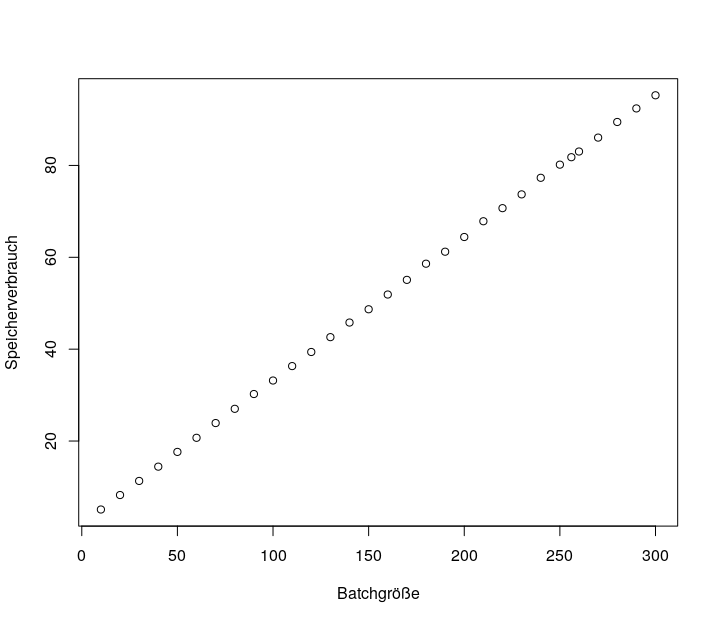
\includegraphics[width= .6\textwidth]{KapitelPartB/Images/memory1.png}\label{abb:memory1}}
     \caption{Experimente zur Batchgröße}
     \label{abb:memory}
\end{figure}
Durch diesen linearen Zusammenhang reicht es ein Modell zu bilden, welches für einen Wert des Speicherverbrauchs abhängig von der Netzarchitektur berechnet, wie groß die Batchgröße maximal sein darf. Zu diesem Zweck wird für ein Netz mit drei Phasen betrachtet und ein Modell entwickelt mit dem sich die maximale Batchgröße berechnen lässt. Die maximale Batchgröße hängt ab von:
\begin{itemize}
 \item der Blockanzahl
 \item der Phasenanzahl und
 \item der Anzahl an Schichten pro Block
\end{itemize}
In Abbildung \ref{abb:memory2} ist abgebildet, wie sich die Blockanzahl auf die Speicherauslastung und auf die maximale Batchgröße auswirken.



\subsection{Evaluierung der Anpassung der Batchgröße an die Netzgröße}






\begin{comment}
Um die Batchgrösse mit der Netzverkleinerung anzupassen muss zunächst die maximale Speicheraulastung und damit die initiale Batchgröße festgelegt werden. In Abbildung \ref{abb:memory1} ist zu sehen, wie sich die Speicherauslastung in Abhängigkeit zur Batchgröße verhält.

\begin{figure}[h]
 \centering
 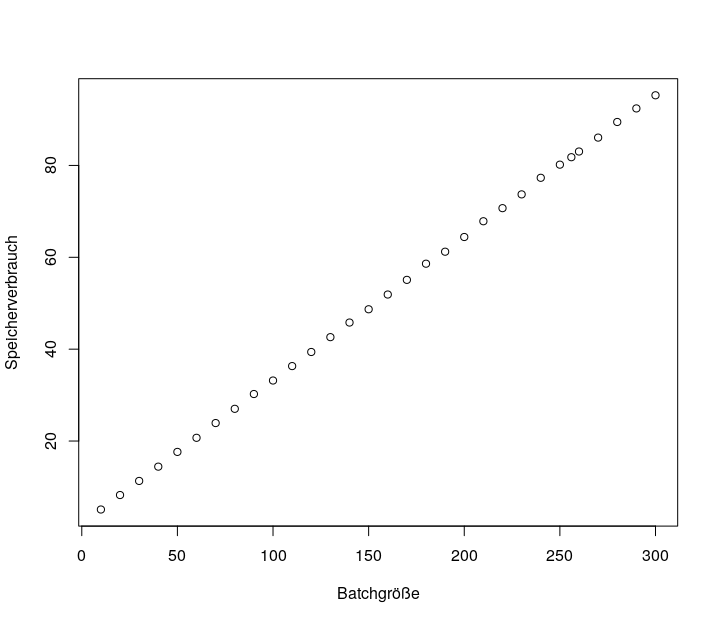
\includegraphics[width=0.8\textwidth]{KapitelPartB/Images/memory1.png}
 % memory1.png: 718x624 px, 96dpi, 19.00x16.51 cm, bb=0 0 539 468
 \caption{Zusammenhang Batchgröße und Speicherverbrauch}
 \label{abb:memory1}
\end{figure}




Dafür wird zunächst untersucht wie sich die Speichernutzung verändert bei unterschiedlich großen Batchgrößen aber fester Netzgröße. Genutzt wird das Basisnetz aus Kapitel \ref{sec:baseline}. 

In Abbildung \ref{abb:}




\begin{table}[]
\begin{tabular}{c|c|c|c|c|c|c|}
\cline{2-7}
     & \multicolumn{2}{c|}{s=1}  & \multicolumn{2}{c|}{s=2}  & \multicolumn{2}{c|}{s=3}    \\ \cline{1-1}
\multicolumn{1}{|l|}{}   & \#Para      & Batch     & \#Para       & Batch     & \#Para & Batch  \\ \hline
\multicolumn{1}{|l|}{1}  & 5306        & 506       & 24090        & 506       \\ \hline
\multicolumn{1}{|l|}{2}  & 9978        & 435       & 47322        & 435       & 434        \\ \hline
\multicolumn{1}{|l|}{3}  & 14650       & 382       & 70554       & 3382        \\ \hline
\multicolumn{1}{|l|}{4}  & 19322       & 339       & 93786        & 339       & 390170      & 301        \\ \hline
\multicolumn{1}{|l|}{5}  & 23994       & 304       & 117018       & 339       & 487386      & 256        \\ \hline
\multicolumn{1}{|l|}{6}  & 28666       & 277       & 140250       & 256       & 584602      & 223        \\ \hline
\multicolumn{1}{|l|}{7}  & 33338       & 256       & 163482       & 229       & 681818      & 198        \\ \hline
\multicolumn{1}{|l|}{8}  & 38010       & 236       & 186714       & 204       & 779034      & 175        \\ \hline
\multicolumn{1}{|l|}{9}  & 42682       & 218       & 209946       & 184       & 876250      & 161        \\ \hline
 \multicolumn{1}{|l|}{10} & 47354      & 205       & 233178       & 171       & 973466      & 147        \\ \hline
\end{tabular}
\end{table}




Gleichzeitig wird für die jeweilige Modellgrösse die Anzahl an Parametern, die das Modell hat gezählt. Diese Größen sind in Tabelle \ref{tab:batchSize} eingetragen. 
\color{black}

Mit Hilfe dieser Grössen wird für jede einzelne Stagegröße eine Gerade gefittet.

Diese gefittete Gerade wird mittels t-Test darauf überprüft wie wahrscheinlich beim Fitten der Gerade ein Fehler 1. Art auftritt.

Hierfür werden folgende Hypothesen aufgestellt:


Da der p-Wert für diese Gerade bei $p=2,911e^{-16}$ und damit weit unter de Signifikanzniveau von $\alpha=0,05$ kann die $H_0$ Hypothese abgelehnt werden und die Alternativhypothese angenommen werden.

Dies bestätigt statistisch eine hohe Wahrscheinlichkeit, dass die gefittete Gerade richtig ist.



In Abbildung \ref{fig:linearBlocks} ist zu sehen, dass die Parameteranzahl in Zusammenhang mit der Anzahl an Blöcken linear steigt.
Wird das Netz kleiner, so kann anhand der Gerade abhängig von der Parameteranzahl die neue Batchgröße errechnet werden.






\todo{beispielrechnung}

In Abbildung \todo{ref} ist abgebildet. wie sich die Trainingszeiten verändern, wenn die Batchgrösse angepasst wird.



\subsubsection{Veränderung der Accuracy durch PruneTrain}

Durch das Pruning währenddem Training wird die Accuracy kleiner. In Abbildung \ref{abb:PTaccuracy} ist zu sehen wie sich im Accuracy im Verlauf der Epochen verändert.  

\begin{figure}[h]
 \centering
 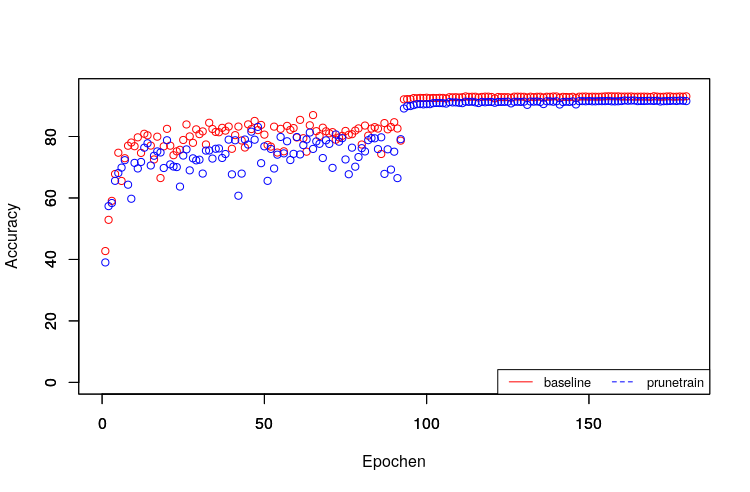
\includegraphics[width=0.8\textwidth]{KapitelPartB/Images/PTaccuracy.png}
 % PTaccuracy.png: 750x492 px, 96dpi, 19.85x13.02 cm, bb=0 0 563 369
 \caption{Veränderung der Accuracy während der Epochen}
 \label{abb:PTaccuracy}
\end{figure}

In Abbildung \ref{abb:PTaccuracyzoom} sind die Epochen 90 bis 180 näher herangezoomt.

\begin{figure}[h]
 \centering
 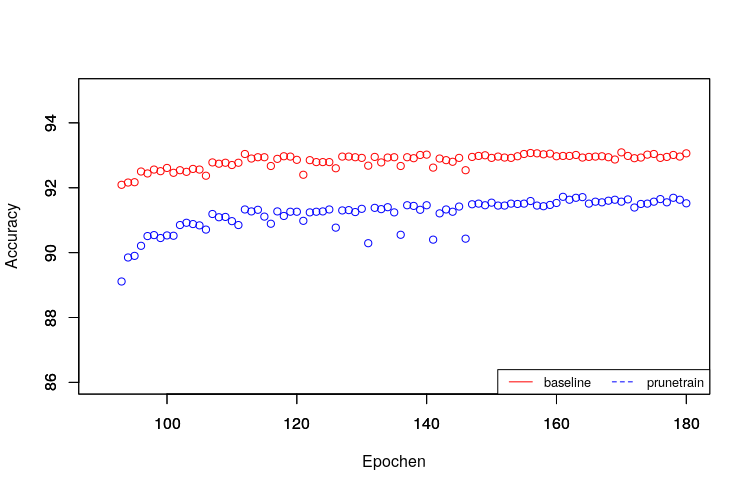
\includegraphics[width=0.8\textwidth]{KapitelPartB/Images/PTaccuracyzoom.png}
 % PTaccuracyzoom.png: 750x492 px, 96dpi, 19.85x13.02 cm, bb=0 0 563 369
 \caption{Zoom der Veränderung}
 \label{abb:PTaccuracyzoom}
\end{figure}

Man sieht eine geringere Accuracy von PruneTrain im Vergleich zum Baseline. Diese Verringerung der Accuracy lässt sich durch ein Aussetzen des Verkleinern des Netzes in den letzten Epochen  
vermindern.

Die Frage die sich hier stellt ist, ob diese Verminderung der Accuracy am Ende der dieser Arbeit noch ins Gewicht fällt. Wenn mit Hilfe einer Kombination von MorphNet und PruneTrain ein bessere Architektur gefunden wird kann diese Architektur auch direkt mit Hilfe des äquivalenten Baseline Netzes berechnet werden.

\subsection{Einfluss der Batchgröße auf PruneTrain}\label{sec:batch}

Das heisst es ist nötig, zu wissen wie gross die Batches maximal sein dürfen um keinen Out of Memory Error zu provozieren. Zusätzlich kann dann berechnet werden, inwieweit die Batchgrösse weiter angehoben werden kann bei kleiner werdendem Netz

Um die Anpassung der Batchgröße an die Verkleinerung des Netzwerkes durch das Prunen zu implmentieren muss zunächst die Batchgröße des Ausgangsnetzes so gewählt werden, dass der GPU-Speicher maximal ausgelastet ist.



Theoretisch sollte hierfür nachdem Übertragen des Modells der freie Speicher ausglesen werden und anhand des Speicherverbrauchs eines Elements des Datensatzes berechnet werden, wie gross die Batchgröße maximal sein darf. Leider führt diese Methode nicht zum gewünschten Ergebnis, da der ausgelesene freie Speicher nicht dem tratsächlich allokierbaren Speicher entspricht.
Der Grund hierfür ist ein Fragmentierungsproblem. Verschiedene freie Blöcke können nicht zu einem grossen allokierbaren Block zusammengefügt werden.\todo[inline]{Quelle}. 

Diese Problem wird mit einer Methode, die für einen beliebigen Datensatz und für eine beliebige Modellgrösse die maximale Batchgröße berechnet, gelöst. 





\begin{figure}[h]
 \centering
 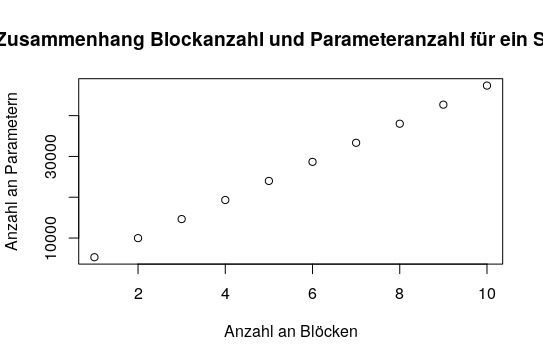
\includegraphics[width=0.8\textwidth]{KapitelPartB/Images/linearBlocks.png}
 % batchSizevsTime.png: 387x367 px, 96dpi, 10.24x9.71 cm, bb=0 0 290 275
 \caption{Batch Size vs Trainings Time über eine Epoche}
 \label{fig:linearBlocks}
\end{figure}




Die maximal mögliche Batchgrösse in Abbildung \ref{fig:maxBatchSize} sinkt im Gegensatz dazu stärker als linear bei mehr Blöcken im Netz. Dies liegt darin begründet, dass für ein grösseres Netz mehr Werte zwischengespeichert werden müssen, was den Speicherbedarf erhöht.

\begin{figure}[h]
 \centering
 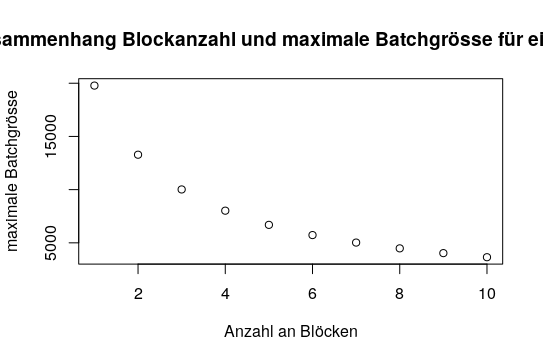
\includegraphics[width=0.8\textwidth]{KapitelPartB/Images/maxBatchSize.png}
 % batchSizevsTime.png: 387x367 px, 96dpi, 10.24x9.71 cm, bb=0 0 290 275
 \caption{Batch Size vs Trainings Time über eine Epoche}
 \label{fig:maxBatchSize}
\end{figure}




Gesucht ist ein idealerweise linearer Zusammenhang zwischen der Parameteranzahl und der Batchgrösse. Um diesen herzustellen wird die Parameteranzahl durch die Batchanzahl geteilt. Das Ergebnis hiervon ist in Abbildung \ref{fig:quotient} zu sehen.

\begin{figure}[h]
 \centering
 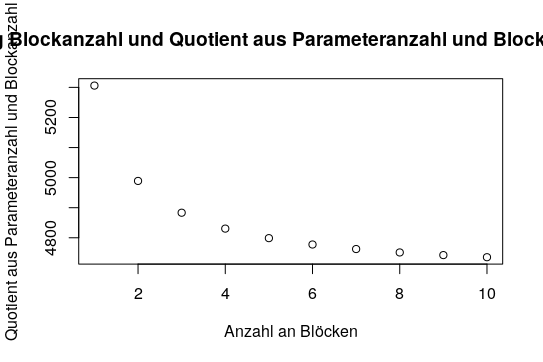
\includegraphics[width=0.8\textwidth]{KapitelPartB/Images/quotient.png}
 % batchSizevsTime.png: 387x367 px, 96dpi, 10.24x9.71 cm, bb=0 0 290 275
 \caption{Batch Size vs Trainings Time über eine Epoche}
 \label{fig:quotient}
\end{figure}


Da diese Kurve ähnlich der Batchsize-Kurve aussieht wird die Hypothese untersucht, ob hier ein linearer Zusammenhang besteht. Zu diesem Zweck wird die Batchgrösse durch das Ergebnis geteilt.

Augenscheinlich liegt hier ein linearer Zusammenhang vor. Daher wird hier eine Gerade gefittet.
Es entsteht die Abbildung \ref{fig:gerade}.

\begin{figure}[h]
 \centering
 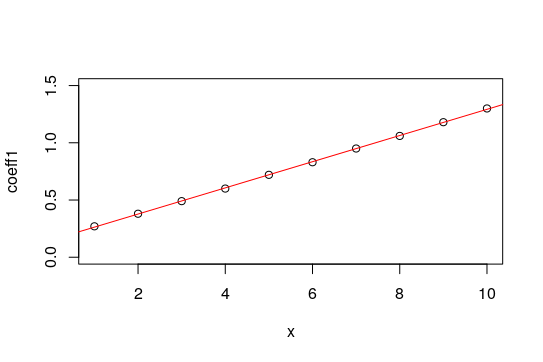
\includegraphics[width=0.8\textwidth]{KapitelPartB/Images/gerade.png}
 % batchSizevsTime.png: 387x367 px, 96dpi, 10.24x9.71 cm, bb=0 0 290 275
 \caption{Batch Size vs Trainings Time über eine Epoche}
 \label{fig:gerade}
\end{figure}




Die gefittete Gerade hat die Gleichung: $$ f(x)=0.11 \cdot x +  0.15 $$

\todo{Hier muss noch das Fitten des Modells und der t-Test erklärt werden}

In Tabelle \todo{Tabelle} werden die Werte für die anderen Stages zusammengefasst. Zu sehen ist, dass für jeden Stage die gefittete Gerade ähnlich im t-Test abschneidet.







Als nächsten Schritt wird untersucht wie das Intervall wie häufig rekonfiguriert wird den Zusammenhang zwischen Inferenz Flop und der Validation Accuracy verändert.


Die nächste Untersuchung über das Sparen von Kommunikationskosten beim Verteilten Training macht hier keinen Sinn da nur eine einzelne Graka genutzt wird.


Abschliessend wird noch evaluiert, wie die Dichte der Gewichte mit der Dichte der Kanäle nachdem Training zusammenhängen um eventuell durch spezifische Inferenzhardware weiter zusparen.





Bei grösserer Batchgrösse wird auch das Netz schneller. Dies ist in Abildung \ref{fig:batchVsTime} für das ResNet und die verwendete Hardware abgebildet.

\begin{figure}[h]
 \centering
 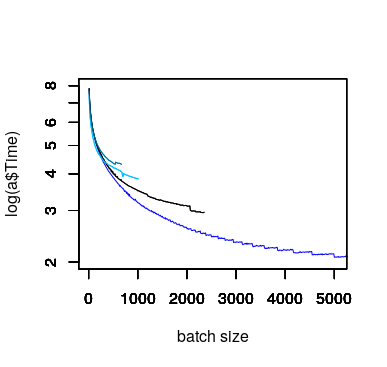
\includegraphics[width=0.8\textwidth]{KapitelPartB/Images/batchSizevsTime.png}
 % batchSizevsTime.png: 387x367 px, 96dpi, 10.24x9.71 cm, bb=0 0 290 275
 \caption{Batch Size vs Trainings Time über eine Epoche}
 \label{fig:batchVsTime}
\end{figure}


Wie zu sehen ist, wird die Trainingszeit pro Epoche mit grösserer Batchgrösse kleiner. Die höhere Batchgrösse sorgt neben der geringeren Trainingszeit auch für weniger Gewichtsupdates. Dies führt zu einer geringeren Generalisationsfähigkeit und damit zu einer geringeren Klassifikationsleistung \cite{largeBatch}. Um diesen Verlust an Klassifikationsleistung auszugleichen gibt es die Möglichkeit die Lernrate anzupassen und eine andere Batch Normalisation zu verwenden \cite{largeBatch}. Diese Technik funktioniert laut dem Paper "`Train longer, generalize better: closing the generalization gap in large batch training of neural networks"' bereits auf residualen Netzen wie sie in dieser Arbeit verwendet werden \cite{largeBatch}. Vorallem bleibt die Einsparung bei der Trainingszeit durch diese Technik intakt \cite{largeBatch}.

Ist dieser Effekt auf PruneTrain übertragbar?


Eine grössere Batchsize sorgt auf jeden Fall für signifikant weniger Verkleinerung des Netzes.

Die Frage die sich hier stellt ist, ob mit Hilfe von largeBatch bei maximaler Batchsize die Verkleinerungsrate steigt  
\end{comment}



\chapter{Evaluierung von Net2Net}\label{sec:net2netexperimente}
Die Operatoren zur Beschleunigung des Lernens durch Wissenstransfer werden in diesem Unterkapiel evaluiert. Diese Evaluierung arbeitet selbst erstellten Implementierung.

Die Evaluierung umfasst drei unterschiedliche Situationen, diese Situation sind analog zu den in der dazugehörigen Quelle \cite{net2net}. Die Evaluierung arbeitet mit einem ResNet, welches auf Cifar10 trainiert wird. In der ersten Situation wird der Operator für ein breiteres Netz verwendet, um ein schmalleres ResNet32 zu trainieren. In der zweiten Situation wird der Operator für ein tieferes Netz benutzt um in einem der Stages des Netzes einen neuen Block einzufügen. In der dritten Situation werden beide Operatoren kombiniiert. Mit der Kombination wird der Raum erkundet, der durch die verschieden tiefen und breiten Modelle aufgespannt wird.
Die drei Situationen werden in den drei folgenden Unterkapiteln näher beschrieben.




\subsection{Evaluierung des Operators für ein breiteres Netz}
Evaluiert wird der operator durch verschiedene Optionen, welche Bereich des Netzes breiter gemacht wird:
\begin{itemize}
 \item Eine ganze Phase
 \item Alle Phasen
\end{itemize}
Wie in Kapitel \ref{sec:net2net} beschrieben werden beim Operator für ein breiteres Netz die Gewichte für die neu hinzugefügten Gewichte aus den ursprünglichen Gewichten berechnet. Um zu evaluieren wie gut diese Methode funktioniert wird sie verglichen mit dem schmallen und breiten Baseline-Netz. Um die Methode der Initialisierung der zusätzlichen Kanäle zu evaluieren wird als Vergleich ein Netz trainiert, bei welchem die zusätzlichen zusätzlichen Gewichte zufällig initialisiert werden.
\subsection{Evaluierung des Operators für ein tieferes Netz}
Zur Evaluierung des breiteren Netzes wird zunächst wie in der Veröffentlichung jeder Block um eine Schicht erweitert. Dabei werden die zusätzlichen Schichten wie in Kapitel \ref{sec:deep} beschrieben initialisiert. Als Vergleich dient das Baseline-Netz aus Kapitel \ref{sec:baseline}.



Eine weitere Verwendung des Operators für ein tieferes Netz ist die Möglichkeit einen neuen Block hinzuzufügen. Nur ein einfaches Hinzufügen würde hier zu Problemen führen. Der Grund hierfür ist Abbildung \ref{abb:deeper} dargstellt. Dabei soll an einer Verbidung, die bisher die Daten von einer Schicht zur nächsten transportiert ein neuer Block inklusive Kurzschlussverbindung entstehen. Der hinzuzfügende Block blau \todo{blau markieren} markiert. Der neue Block soll wie die Kurzschlussverbindung die Identität berechnen. Betrachtet $x$ als Größe der Identität. Dann wird hier mit dem neuen Block staat $x$ das doppelte, also $``X$ berechnet. Um dieses Problem zu umgehen wird an jeder Additionsstelle für eine Kurzschlussverbindung eine Multiplikation mit 0,5 berechnet (rechte Seite der Grafik). So wird nicht mehr $x$ sondern $0,5x +0,5=x$ berechnet.  


\begin{figure}[h]
 \centering
 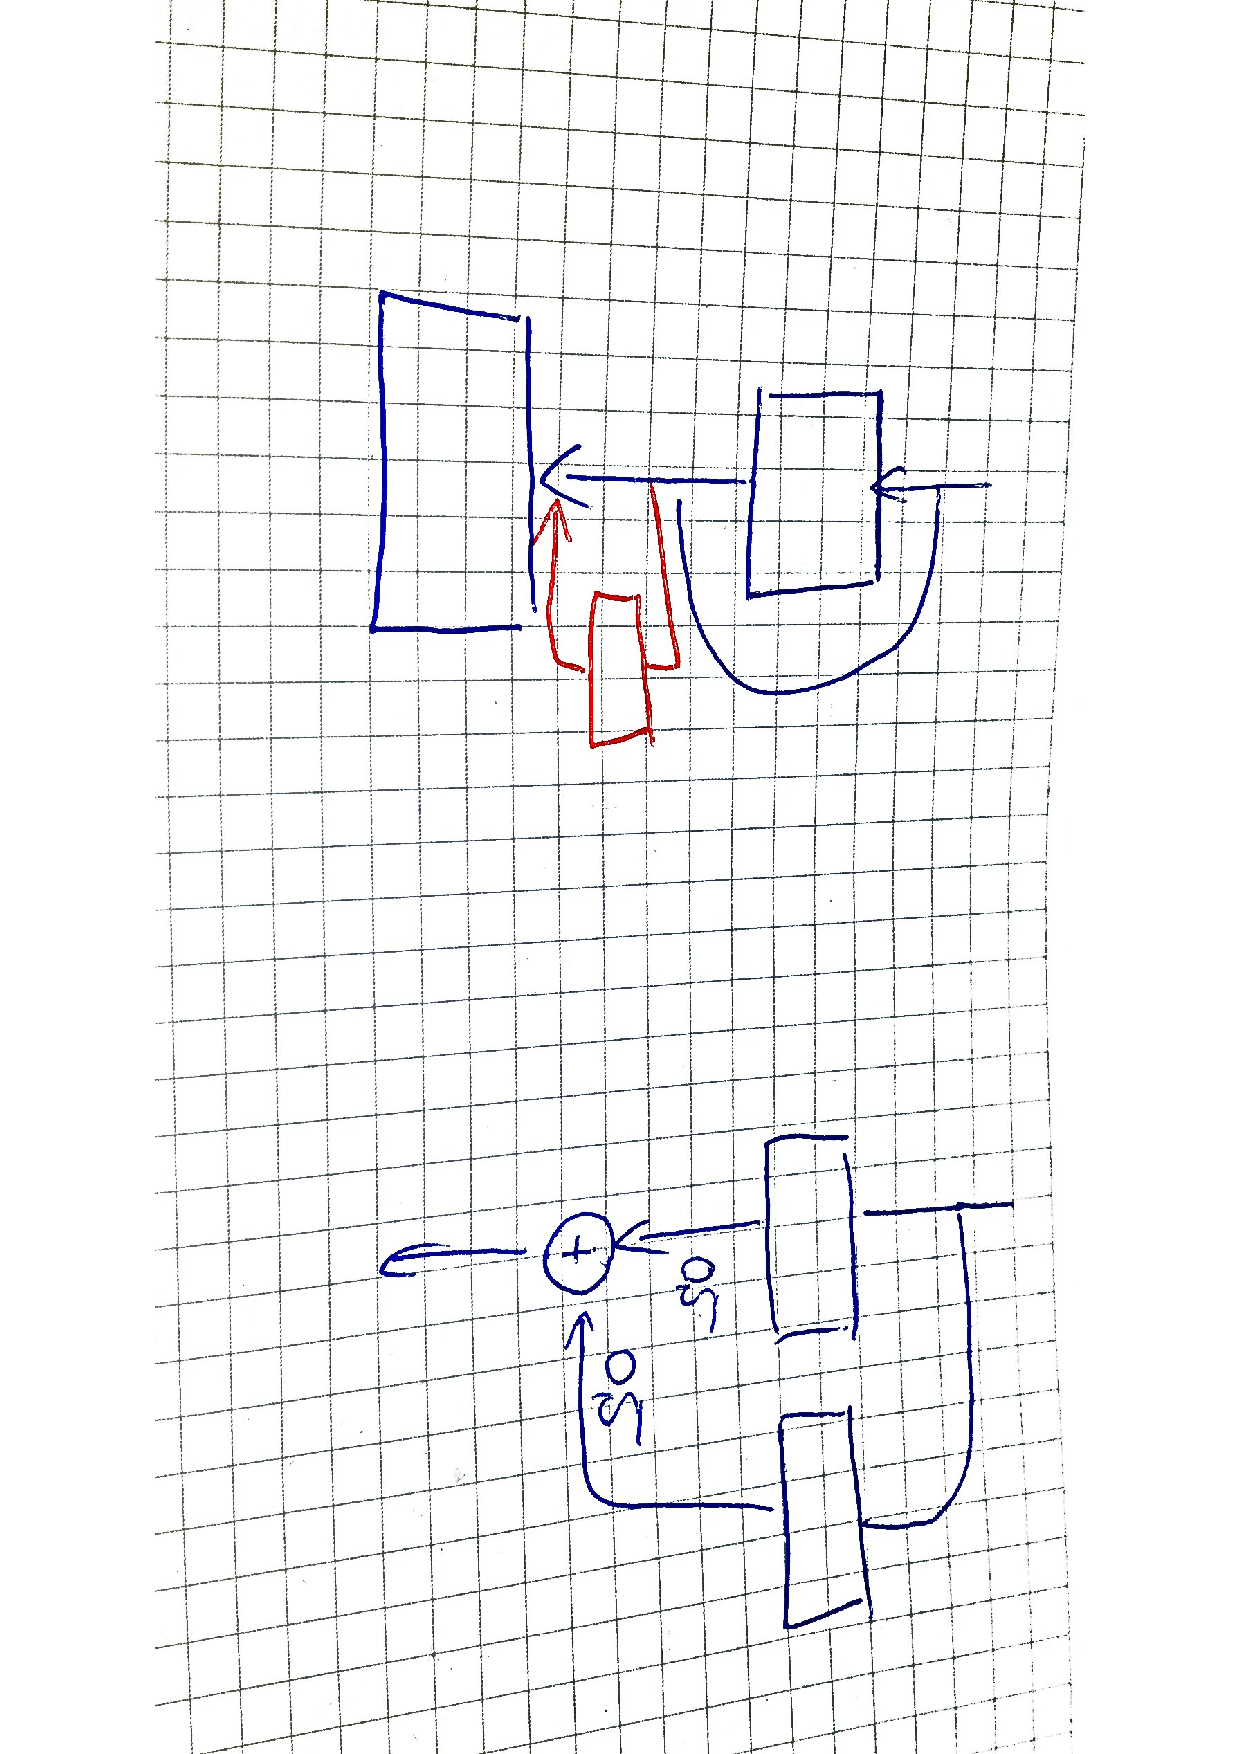
\includegraphics[width=0.5\textwidth, angle=90]{KapitelPartB/Images/deeper.pdf}
 % deeper.pdf: 0x0 px, 300dpi, 0.00x0.00 cm, bb=
 \label{abb:deeper}
\end{figure}




\subsection{Erkunden des Modellraums}



\chapter{Evaluierung }\label{sec:ptpnet2net}
Adaptive Kombination of prune and net2net

AKoPaN

Für die Kombination betrachten wir zunächst den Ausgang eines PruneTrain-Durchlaufs über 180 Epochen mit verschieden breiten Netzen:

4,8,16


8,16,32


16,32,64


und verschieden tiefen Netzen:

[3,3,3]


[4,4,4]




Gestartet wird wie bei Morphnet einmal mit 


4,8,16 und mit 


8,16,32
jeweils mit 3 Blöcken pro Phase
anlaog zu Kapitel 4.


um das Grösserwerden des Netzes nicht ausarten zu lassen sollte es nicht größer werden als 
das [5,5,5] er Netz mit 16,32,64 als maximalen Größe vorgegeben.




Drei Probleme können beim Training des Ntzes auftauchen:
\begin{itemize}
 \item Underfitting
 \item Overfitting
 \item Saturation
 \item Rumspringen ohne eine Tendenz zur Verbesserung
\end{itemize}

Underfitting erkennen wir durch einen immer noch recht hohen Trainingsfehler und relativ wenig Pruning.


Sowohl bei Hinzufügen von neuen Blöcken als auch beim Breiter machen des Netzes kann Overfitting passieren. Kommt es zu Overfitting ist es möglich, den Lasso-Ratio koeffizient weiter zu erhöhen, oder den Grenzwert zum Beschneiden des Netzes zu Erhöhen. Das heisst es ist nötig, Overfitting zu erkennen. Dies wird hier durch Abstand von Trainings und Validierungsfehler. Wird der Abstand hier grösser bei einer Zunnahme des Validierungsfehlers oder  ist die Testaccuracy bei 100 \% angekommen, wird Overfitting diagnostiziert.


Saturation
Bilde aus den letzten 10 Validierungsaccuracy jeweils ein exponentiel geglättetes Mittel gewichtetes Mittel. Zeigt dieses Mittel keine Verbesserung innerhalb der nächsten 10 Epochen -> early stop und je nach vorliegen von Under oder Overfitting weiterverfahren.

\subsection{Exponentiell gleitender Durchschnitt}
Der exponentiell gleitende Durchschnitt ist eine Möglichkeit eines leitenden Durchschnitts mit mehr Gewicht je neuer eine Messung ist. In Abbildung \ref{abb:egd} ist zu sehen, wie sich dieser für die Validierungsaccuracy des Baseline Netzes verhält.

\begin{figure}[h]
 \centering
 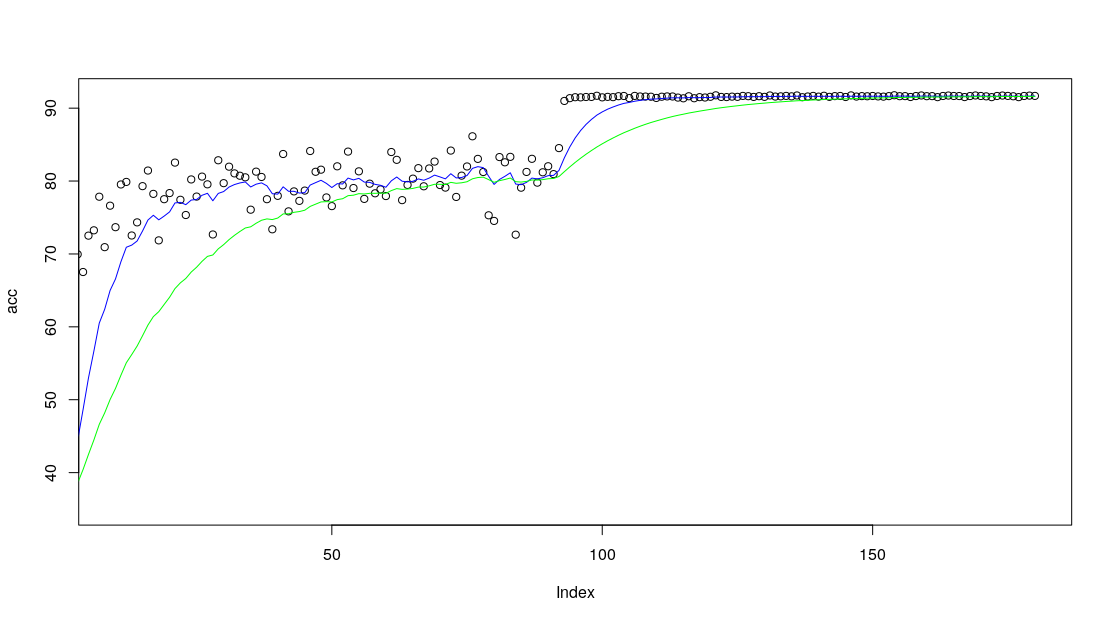
\includegraphics[width=0.8\textwidth]{KapitelPartB/expmean.png}
 % expmean.png: 1112x623 px, 96dpi, 29.43x16.49 cm, bb=0 0 834 467
 \caption{Exponentiell geglätteter Durchschnitt}
 \label{abb:egd}
\end{figure}

Dabei sind 2 Effekte zu sehen:
1. ab Epoche 150 passiert so gut wie nichts mehr: die Term der exp glättung ist waagerecht
2. ab Epoche 80 ist es nur ein Rumspringen.

In beiden Fällen kann Abhilfe geschaffen werden: Versuche zunächst für 30 Epochen die Lernrate weiter zu senken. Wenn sich nach diesen 30 Epochen immer noch die beiden gleitenden Mittelwerte gleich sind:







\chapter{Vergleich}\label{sec:vergleich}

\begin{comment}
\chapter{Additive Verfahren}

\subsection{Zahlenformate}\label{sec:zahlen}
\todo[inline]{Text fertig schreiben; etwa 4 Stunden}
\begin{itemize}
 \item FP16 bereits probiert
\end{itemize}


FP16 nur auf RTX 2080 sinnvoll
Bietet nach erster Messung etwa 28 \% Prozent Gewinn.

Code für dieses Verfahren liegt vor: Amp apex von Nvidia

AMP bietet 3 mögliche Optimierungsstufen:

O1
Patch all Torch functions and Tensor methods to cast their inputs according to a whitelist-blacklist model. Whitelist ops (for example, Tensor Core-friendly ops like GEMMs and convolutions) are performed in FP16. Blacklist ops that benefit from FP32 precision (for example, softmax) are performed in FP32. O1 also uses dynamic loss scaling, unless overridden.

02
casts the model weights to FP16, patches the models forward method to cast input data to FP16, keeps batchnorms in FP32, maintains FP32 master weights, updates the optimizer’s paramgroups so that the optimizer.step() acts directly on the FP32 weights (followed by FP32 master weight-FP16 model weight copies if necessary), and implements dynamic loss scaling (unless overridden). Unlike O1, O2 does not patch Torch functions or Tensor methods.


O3
may not achieve the stability of the true mixed precision options O1 and O2. However, it can be useful to establish a speed baseline for your model, against which the performance of O1 and O2 can be compared. If your model uses batch normalization, to establish speed of light you can try O3 with the additional property override keepBatchnormfp32=True (which enables cudnn batchnorm, as stated earlier).

Hier nur O0, O1 und O2 dargestellt, da O3 absolut nicht mithalten kann was Performance angeht.

\begin{figure}[h]
 \centering
 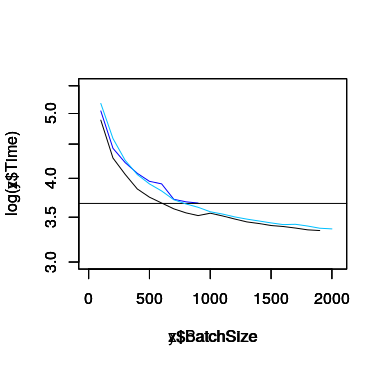
\includegraphics[width=0.8\textwidth]{KapitelPartB/Images/timeVsBatchSize_Amp.png}
 % timeVsBatchSize_Amp.png: 387x367 px, 96dpi, 10.24x9.71 cm, bb=0 0 290 275
 \caption{Vergleich Trainingszeit einer Epoche für verschiedene Optimierungsstufen von Amp Apex. DunkelBlau=O0; Schwarz = O1; Hellblau=O2}
 \label{fig:amp}
\end{figure}
\url{https://developer.download.nvidia.com/video/gputechconf/gtc/2019/presentation/s9998-automatic-mixed-precision-in-pytorch.pdf} zeigt, dass bezüglich der Accuracy kein Verlust zu erwarten ist.

Da O2 gegenüber O1 keinen signifikanten zusätzlichen Gewinn bringt nutze O1.



\subsection{LARS}\label{sec:lars}
\todo[inline]{Experimente fast fertig (3x mal auf einer Graka für 50 min); dann etwa 3 Stunden fürText + Evaluierung}




Es stellt sich die Frage, ob das einen so grossen Einfluss auf die Ausführungszeit hat.



Man sieht, dass mit steigender Batchgröße die Ausführungszeit sinkt. 

Errechne zusätzlich noch ein Modell, wo abhängig von der Modellgrösse währenddem Pruning die Batchgrösse angepasst wird.





\subsection{Beschleunigung der Berechnung des Gradientenabstiegverfahren}
\todo[inline]{ab hier löschen}

Accelerating CNN Training by Sparsifying Activation Gradients funktioniert nur auf Toy-Benchmarks 


\subsubsection{Weight Normalization: A Simple Reparameterization
to Accelerate Training of Deep Neural Networks}


Könnte funktionieren. Code für Lasagne: https://github.com/TimSalimans/weight\_norm


\subsubsection{Accelerating Deep Neural Network Training with Inconsistent Stochastic Gradient Descent}

Interessant bisher kein Code verfügbar

\subsubsection{Accelerated CNN Training Through Gradient Approximation }

Interessant bisher kein Code verfügbar


\end{comment}
